% =============================================================================
% 5‑Body.tex — State of the Art, General Description, Implementation, Results
% =============================================================================

% ╔═══════════════════════════════════════════════════════════════════════════╗
% ║  Chapter 2 — State of the Art                                           ║
% ╚═══════════════════════════════════════════════════════════════════════════╝
\chapter{State of the Art}
\label{ch:state-of-art}

\section{PID Control}
\label{sec:sota-pid}

\section{Fuzzy Logic and Fuzzy Control}
\label{sec:sota-fuzzy}

\section{Depth-First Search for Maze Solving}
\label{sec:sota-dfs}

% ╔═══════════════════════════════════════════════════════════════════════════╗
% ║  Chapter 3 — General Description                                        ║
% ╚═══════════════════════════════════════════════════════════════════════════╝
\chapter{General Description}
\label{ch:general-description}

\section{System Overview}
\label{sec:system-overview}

\section{Hardware Configuration}
\label{sec:hardware}

\section{Software Architecture}
\label{sec:software-arch}

% ╔═══════════════════════════════════════════════════════════════════════════╗
% ║  Chapter 4 — Implementation                                             ║
% ╚═══════════════════════════════════════════════════════════════════════════╝
\chapter{Implementation}
\label{ch:implementation}

% ─────────────────────────────────────────────────────────────────────────────
% 4.1  LANE KEEPING
% ─────────────────────────────────────────────────────────────────────────────
\section{The Lane Keeping Module}
\label{sec:lane-keeping}

\subsection{Task Description}
\label{sec:lk-task}

This project implements a robust algorithm in which the LEGO Mindstorms EV3 follows a trajectory on a white surface that is bordered with the help of two black lines between which the robot is situated, thus keeping itself in a lane.

Previous diploma projects including Mindstorms EV3 included the task of following a single black line. The purpose of the robot was to make correction turns when the sensor attached to it began to read another value other than the one of the black line. With the help of proportional, integral and derivative gains, the turns are adjusted from gentle turns to harsh ones.

So, unlike traditional robots that follow a single line this project focuses on a robot that uses two color sensors to balance itself inside the white ``road'' that is contrasted with the two black edges. It utilizes a custom controller combined with an emergency safety net to achieve a reliable and smooth navigation.

The robot is evaluating continuously its physical position by computing how far it has drifted from the ideal center and applying corrective steering to maintain its trajectory. In doing so, the robot uses two color sensors on each side of its front which adjust it from a disturbed state to an ideal state.

The Ideal State, described in the code by the variable setpoint, is the state in which the robot is perfectly centered, and both sensors read the exact reflection value from the white, meaning the difference is 0.

The Disturbed State is the state where the robot, by drifting left or right, moves over the black boundary line. This causes the sensor's value on the black line to drop while the other sensor remains on white, so it keeps its value. In this situation, the difference between the two sensors becomes non-zero and it needs to be fed to control algorithms to be corrected.

The task configuration defines the following thresholds:

\begin{lstlisting}[language=Python, caption={Lane keeping task configuration.}, label={lst:lk-config}]
if task == "LaneKeeping":
    taskConfiguration={
        "LeftColorSensor":    Port.S2,
        "RightColorSensor":   Port.S3,
        "BlackThreshold":     6,
        "CrossingThreshold":  7,
        "MinDifference":      3,
        "BaseSpeed":          90,
        "TurningSpeed":       60,
        "EmergencySpeed":     30,
        "EmergencyTurnSpeed": 45,
        "StopConfirmCount":   1,
        "LogInterval":        1,
    }
\end{lstlisting}

The Left and Right Color Sensors are connected to the physical ports of the robot. The \texttt{BlackThreshold} represents value 6 where the sensors are above the black line, while \texttt{CrossingThreshold} represents the value 7 where the sensors are very close to the black line. The \texttt{MinDifference} being 3 represents the tolerance zone where the sensors are above white surface, but they don't read the exact same value (values close to 0 means dark and values close to 100 means bright). This allows the robot to continue straight, ignoring shadows on the white surface. The \texttt{BaseSpeed} is the forward velocity of the robot being perfectly centered. It is 90 mm/s since the track isn't long and can be easily followed. The \texttt{TurningSpeed} being 60 mm/s is the reduced forward velocity of the robot during a regulation to prevent the robot from overshooting its turns. The \texttt{EmergencySpeed} (30 mm/s) and \texttt{EmergencyTurnSpeed} (45 deg/s) are highly restrictive forward speed, respectively extreme rotational speed, used exclusively to aggressively pivot the robot away from a lane exit. The \texttt{StopConfirmCount} is the number of times the robot detects the value of black on both sensors before it stops. Due to false readings caused by shadows or oversteering in narrow corridors, this variable has been introduced. After many runs of the robot when there were no more false readings, the value of times it encounters black is set to 1. The \texttt{LogInterval} is the number of seconds to pass to print what the robot has recorded and what action did it took. It is 1 for a more detailed log.

\subsection{The Lane Keeping Controller}
\label{sec:lk-controller}

The Lane Keeping application’s functionality is described in the \texttt{LaneKeepingController} class, which implements the \texttt{Controller} interface. In this class there are defined the methods which contribute to the desired behavior of the robot when it tries to follow the lane. It firstly initializes the attributes in the constructor, retrieves the values from the sensors, prints the header of the log, decides what action needs to be taken and finally the run method which starts the robot to move.

\begin{lstlisting}[language=Python, caption={LaneKeepingController constructor.}, label={lst:lk-init}]
def __init__(self, algorithm, configuration, streamer, ev3, robot):
    super().__init__(algorithm, configuration, streamer, ev3, robot)
    self.leftSensor=ColorSensor(configuration["LeftColorSensor"])
    self.rightSensor=ColorSensor(configuration["RightColorSensor"])
    self.blackThreshold=configuration["BlackThreshold"]
    self.crossingThreshold=configuration["CrossingThreshold"]
    self.minDifference=configuration["MinDifference"]
    self.baseSpeed=configuration["BaseSpeed"]
    self.turningSpeed=configuration["TurningSpeed"]
    self.emergencySpeed=configuration["EmergencySpeed"]
    self.emergencyTurnSpeed=configuration["EmergencyTurnSpeed"]
    self.stopConfirmCount=configuration["StopConfirmCount"]
    self.logInterval=configuration["LogInterval"]
\end{lstlisting}

The constructor takes the inherited attributes from the super abstract class \texttt{Controller} and along with the more specific attributes taken from the \texttt{configuration} dictionary. These attributes initialize the state of the \texttt{LaneKeepingController} object.

\begin{lstlisting}[language=Python, caption={LaneKeepingController sensors reading.}, label={lst:lk-init}]
def readSensors(self):
    leftValue=self.leftSensor.reflection()
    rightValue=self.rightSensor.reflection()
    return leftValue, rightValue
\end{lstlisting}

This method simply reads the values of the light reflected on the surface they are currently on and returns them.

\begin{lstlisting}[language=Python, caption={LaneKeepingController header printing.}, label={lst:lk-init}]
def printHeader(self, algorithm):
    self.ev3.speaker.beep()
    print("\nLANE KEEPING-"+algorithm+"\n")
    print("Black Threshold:"+ str(self.blackThreshold))
    print("Crossing Threshold:"+ str(self.crossingThreshold))
    print("Min Difference:"+ str(self.minDifference))
    print("Base Speed:"+ str(self.baseSpeed))
    print("Turning Speed:"+ str(self.turningSpeed))
    print("Emergency Speed:"+ str(self.emergencySpeed)+"\n")
\end{lstlisting}

This method prints the header of the log to be able to compare the results and see how the thresholds affect the decision-making process after the run.

\begin{lstlisting}[language=Python, caption={LaneKeepingController action deciding.}, label={lst:lk-init}]
def decideAction(self, leftValue, rightValue, difference, dt):
    if leftValue<self.crossingThreshold and rightValue>=self.crossingThreshold:
        return self.emergencySpeed, self.emergencyTurnSpeed
    
    if rightValue<self.crossingThreshold and leftValue>=self.crossingThreshold:
        return self.emergencySpeed, -self.emergencyTurnSpeed
    
    if abs(disturbance)<=self.minDifference and isinstance(self.algorithm, (PIDAlgorithm, FuzzyPIAlgorithm)):
        return self.baseSpeed, 0
    
    disturbance, turnRate=self.algorithm.compute(0, disturbance, dt)
    
    return self.turningSpeed, turnRate
\end{lstlisting}

This method implements a safety layered architecture with three priority levels: emergency override, admitted tolerance and algorithm regulation. Based on this architecture, the method decides what action needs to be taken based on the values read by the sensors and the difference between them. 

The first case treats the moment when the left sensor reads a value close to the black and the right sensor reads a larger value. This means that the robot is crossing the black line on the left side, so the method returns the emergency speed and the emergency turn speed with positive value, meaning turning right. 

The second case is opposite to the first as it treats the moment when the right sensor reads a value close to the black and the left sensor reads a larger value. This means that the robot is crossing the black line on the right side, so the method returns the emergency speed and the emergency turn speed with negative value, meaning turning left. 

The third case treats the difference with the values of the sensors being smaller or equal than the minimum difference accepted to let the robot continue straight ahead, meaning that the robot is on a bright surface and the method returns the normal speed and the speed of turning is 0 to move without deviation. This case is only applied for the PID and Fuzzy PI algorithms since the Fuzzy Rule-Based algorithm can have rules that apply even when the robot is close to the center.

In the fourth case the disturbance and turn rate are taken from the results done by the compute() method of the selected algorithm. The method finally returns the turning speed and the turn rate (the output of the regulation) meaning that the robot is regulated by the selected algorithm.

\begin{lstlisting}[language=Python, caption={LaneKeepingController main run loop.}, label={lst:lk-init}]
def run(self):
    self.printHeader(self.algorithmLabel())
        
    bothSensorsOnLineCount=0
    lastTime=0.0
    
    try:
        while True:
            step, currentTime=self.nextStep()
            dt=currentTime-lastTime
            lastTime=currentTime
            
            leftValue, rightValue=self.readSensors()
            
            leftOnBlack=leftValue<self.blackThreshold
            rightOnBlack=rightValue<self.blackThreshold
            
            if leftOnBlack and rightOnBlack:
                bothSensorsOnLineCount+=1
                if bothSensorsOnLineCount>=self.stopConfirmCount:
                    self.robot.stop()
                    self.ev3.speaker.beep()
                    print("\nBoth sensors on line for "+str(self.stopConfirmCount)+" consecutive steps. Stopping.")
                    break
                
                self.robot.drive(10, 0)
                wait(20)
                continue
            else:
                bothSensorsOnLineCount=0
                
            disturbance=leftValue-rightValue
            speed, turnRate=self.decideAction(leftValue, rightValue, disturbance, dt)
            self.streamer.send(self.step, disturbance, turnRate)
            self.logger.log(self.step, disturbance, turnRate)
            
            if step%self.logInterval==0:
                print("Step "+str(step)+" Left: "+str(leftValue)+" Right: "+str(rightValue))
                if isinstance(self.algorithm, FuzzyRuleBased):
                    print(self.algorithm.logRules())
            
            if speed<30:
                speed=30
                
            self.robot.drive(speed, turnRate)
            wait(20)
            
    except KeyboardInterrupt:
        self.robot.stop()
        self.ev3.speaker.beep()
        print("\nLANE KEEPING STOPPED\n")
    finally:
        self.streamer.close()
        self.logger.close()
\end{lstlisting}

The final run() method is the main execution loop. It combines four phases of the control cycle: sense, decide, actuate and wait. It includes the previous three methods to execute the task. Firstly, it prints the header according to the algorithm returned by the \texttt{algorithmLabel()} method where its instance was checked and the constants and resets the number of times both sensors crossed the black line and the time.

The continuous loop begins with the computation of the change in time by subtracting the current time (obtained from the \texttt{now()} method) with the last time and updating the last time. The left and right values are assigned with the values read by the sensors and then, based on the log interval, which in this case is 1, is printed at each multiple of it the step plus what values the sensors read. If the algorithm is Fuzzy Rule Based, the rules are also printed.

With the help of the Boolean variables \texttt{leftOnBlack} and \texttt{rightOnBlack}, the condition for the robot to stop is created by having both values of the sensors smaller than the threshold value which indicates a very dark surface. In the event of false readings, the number of times both sensors were on the black line increases until it reaches the confirmation count to stop, otherwise it reduces the speed and waits to see if indeed is on a black line or not.

If the conditions fail, the disturbance is computed and the speed with the turn rate are given by the action it needs to be decided based on the left value, right value, disturbance and the change in time. The returned speed can’t get lower than 10 and the robot is driving based on the final speed and turn rate. The final wait is used to ensure that the loop frequency remains consistent regardless of which branch was taken. 

The except part of the try-except black where the program is interrupted by the user. The robot stops and the stream with the file are closed.

\subsection{PID Algorithm}
\label{sec:pid}

One possible option for the robot to succeed in following the lane is with the help of a PID controller. This algorithm that implements this type of controller uses Comparative Control, where the disturbance of the two color sensors, is computed at each step in order to be given as input to the controller so that it can generate the turn rate so that the disturbance is minimized.

\begin{lstlisting}[language=Python, caption={PIDAlgorithm constructor.}, label={lst:lk-init}]
def __init__(self, configuration):
    self.kp=configuration["Kp"]
    self.ki=configuration["Ki"]
    self.kd=configuration["Kd"]
    self.minOutput=configuration["MinOutput"]
    self.maxOutput=configuration["MaxOutput"]
    self.integralMin=configuration["IntegralMin"]
    self.integralMax=configuration["IntegralMax"]
    self.integral=0.0
    self.previousDisturbance=0.0
\end{lstlisting}

In the first part of the definition of the class, the constructor initializes the constants which will be computed to determine the final turn rate, as well as the interval ends for it and the integral. The previous disturbance and the integral are set to 0.

\begin{lstlisting}[language=Python, caption={PIDAlgorithm compute method.}, label={lst:lk-init}]
def compute(self, setPoint, measuredPoint, dt):
    disturbance=setPoint-measuredPoint
    pTerm=self.kp*disturbance
    
    if dt>0:
        self.integral+=disturbance*dt
        
        if self.integral>self.integralMax:
            self.integral=self.integralMax
        elif self.integral<self.integralMin:
            self.integral=self.integralMin
    iTerm=self.ki*self.integral
    
    if dt>0:
        derivative=(disturbance-self.previousDisturbance)/dt
    else:
        derivative=0.0
        
    dTerm=self.kd*derivative
    
    output=pTerm+iTerm+dTerm
    
    if output>self.maxOutput:
        output=self.maxOutput
    elif output<self.minOutput:
        output=self.minOutput
        
    self.previousDisturbance=disturbance
    
    return disturbance, output
\end{lstlisting}

The \texttt{compute()} method takes the \texttt{setPoint}, which is usually 0 indicating perfect balance between sensors, the \texttt{measuredPoint} which is the actual difference between sensors, and the change in time. The disturbance is the result of ideal minus actual. The final turn rate output is the sum of the three PID terms made of the imbalance and their gains:

\begin{equation}
    \text{Turn Rate} = \bigl(K_P \times \text{Imbalance}\bigr)
    + \left(K_I \times \int \text{Imbalance}\, dt\right)
    + \left(K_D \times \frac{d(\text{Imbalance})}{dt}\right)
\end{equation}

The Derivative Gain symbolizes the present as it only considers the current value of the Disturbance. As the main steering force, its effect on the robot is that the further the robot is from the center, the harder it turns. In other words, if the robot is sluggish and goes off the track on curves, increase the $K_P$. If the robot shakes violently back and forth, decrease the $K_P$. In the \texttt{compute()} method the proportional term is the product of the disturbance and the gain.

The Integral Gain represents the memory since it accumulates the Disturbance over time. If the robot has a mechanical drift, for example a slightly weaker motor, or is on a long, sweeping curve, $K_P$ alone might leave the robot off-center while $K_I$ builds slowly steering power until the robot is perfectly centered. Usually this constant is very small, less than 0.1. Otherwise, it creates Integral Windup, meaning that the robot will overreact drastically and swing off the lane. In the \texttt{compute()} method the integral term is the product of gain and the disturbance multiplied with the change in time, constrained by the integral interval in order to prevent the integral from growing infinitely large.

The Derivative Gain is the dampener as it computes how fast the Disturbance is changing. When the robot steers back toward the center of the lane, $K_D$ acts as a brake. It reduces the steering power right before the robot reaches the center, preventing it from overshooting into the other black line. A higher $K_D$ will tighten the path so that the robot will avoid crawling widely as a snake down the lane. In the \texttt{compute()} method the derivative term is the product of the gain and the derivative of the disturbance with respect to the time.

The output final turn rate is comprised of all three PID terms and restricted to the output interval so that the motors of the robot don’t receive impossible commands.

\begin{lstlisting}[language=Python, caption={PIDAlgorithm reset method.}, label={lst:lk-init}]
def reset(self):
        self.integral=0.0
        self.previousDisturbance=0.0
\end{lstlisting}

The previous disturbance is updated with the current one and the method returns the disturbance and the output. The PIDAlgorithm class also has a reset method to clear the memory of the controller by setting the integral and the previous disturbance to 0.

\subsection{Fuzzy PI Algorithm}
\label{sec:fuzzy-pi}

This algorithm stands apart from a rigid mathematical model as the PID controller by acting as a human driver who adjusts the steering power based on how off the center the robot is. A Fuzzy PI controller changes the constants $K_P$ and $K_I$ depending on the state of the robot using Fuzzy Logic. 

In standard programming the logic is binary, where conditions are either true (1) or false (0). Fuzzy Logic introduces degrees of truth, allowing the robot to categorize a disturbance slightly off-center or very far off-center. By translating the crisp value of the Disturbance into fuzzy sets, the algorithm adjusts dynamically the proportional and integral gains to generate the final turn rate.

\begin{lstlisting}[language=Python, caption={FuzzyPIAlgorithm constructor.}, label={lst:lk-init}]
def __init__(self, configuration):
    self.baseKp=configuration["BaseKP"]
    self.baseKi=configuration["BaseKI"]
    self.smallDisturbance=configuration["SmallDisturbance"]
    self.mediumDisturbance=configuration["MediumDisturbance"]
    self.largeDisturbance=configuration["LargeDisturbance"]
    self.fuzzyMinOutput=configuration["FuzzyMinOutput"]
    self.fuzzyMaxOutput=configuration["FuzzyMaxOutput"]
    self.fuzzyIntegralMin=configuration["FuzzyIntegralMin"]
    self.fuzzyIntegralMax=configuration["FuzzyIntegralMax"]
    self.rules=configuration["Rules"]  
    self.integral=0.0
\end{lstlisting}

The \texttt{FuzzyPIAlgorithm} class implements the fuzzy PI algorithm following the three stages of a fuzzy control system: fuzzification, fuzzy inference and defuzzification. The fuzzification is the conversion of a crisp numerical value into a fuzzy set. The fuzzy inference is the approximate reasoning to formulate a mapping from premise to conclusion. The defuzzification is the reverse conversion of a fuzzy set into a crisp value. The constructor of the fuzzy PI algorithm initializes the base gains $K_P$ and $K_I$ which will be computed to determine the final turn rate, the fuzzy set boundaries S=3, M=6, L=10 describing the disturbance, the rule tuples that encode the gain multipliers for each fuzzy set.

\subsubsection{Fuzzification}

\begin{lstlisting}[language=Python, caption={FuzzyPIAlgorithm fuzzification.}, label={lst:lk-init}]
def fuzzifyDisturbance(self, disturbance):
    disturbanceAbs=abs(disturbance)
    
    if disturbanceAbs<=self.smallDisturbance:
        muSmall=1.0
    elif disturbanceAbs<=self.mediumDisturbance:
        muSmall=(self.mediumDisturbance-disturbanceAbs)/(self.mediumDisturbance-self.smallDisturbance)
    else:
        muSmall=0.0
        
    if disturbanceAbs<=self.smallDisturbance:
        muMedium=0.0
    elif disturbanceAbs<=self.mediumDisturbance:
        muMedium=(disturbanceAbs-self.smallDisturbance)/(self.mediumDisturbance-self.smallDisturbance)
    elif disturbanceAbs<=self.largeDisturbance:
        muMedium=(self.largeDisturbance-disturbanceAbs)/(self.largeDisturbance-self.mediumDisturbance)
    else:
        muMedium=0.0
        
    if disturbanceAbs<=self.mediumDisturbance:
        muLarge=0.0
    elif disturbanceAbs<=self.largeDisturbance:
        muLarge=(disturbanceAbs-self.mediumDisturbance)/(self.largeDisturbance-self.mediumDisturbance)
    else:
        muLarge=1.0
        
    return muSmall, muMedium, muLarge
\end{lstlisting}

The \texttt{fuzzifyDisturbance()} method takes the crisp value of the disturbance and computes the membership degree for each fuzzy set: small $S$, medium $M$ and large $L$. The $\mu_S$, $\mu_M$, $\mu_L$, representing the membership degrees, are values between 0 and 1 and describe how much the input resembles each set simultaneously.

The three fuzzy sets are defined by triangular and trapezoidal membership functions. They are delimited by the boundary values from the configuration: S=3.0, M=6.0 and L=10.0. These boundaries determine where one fuzzy set begins and another ends, with overlapping regions where the disturbance partially belongs to two sets at the same time.  It checks for each fuzzy set because there can be more than one non-zero membership value, and that’s why the method returns all three membership values.

\begin{figure}[htbp]
    \centering
    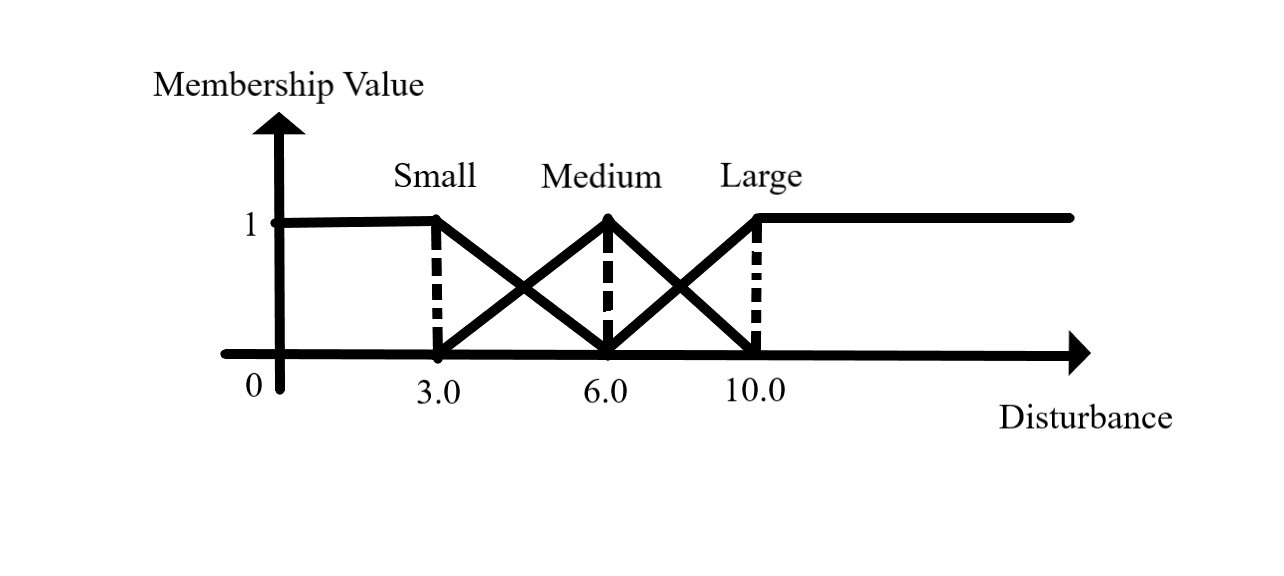
\includegraphics[width=0.7\textwidth]{images/FuzzifyPI.jpg}
    \caption{Fuzzy membership functions for Small, Medium and Large disturbance sets with boundary values $S=3.0$, $M=6.0$ and $L=10.0$.}
    \label{fig:membership-functions-pi}
\end{figure}

The picture above presents graphically the intervals where the disturbance can be situated and what membership value can have, describing a triangular/trapezoidal transition. The disturbance grows or is reduced resulting in smaller membership function for the initial set and a higher membership function for the next set.

For \textit{Small}, a trapezoidal membership function, has full membership ($\mu_S = 1.0$) when $|d| \leq S$. It then decreases linearly from 1 to 0 as the disturbance increases from $S$ to $M$. Zero membership ($\mu_S = 0.0$) when $|d| \geq M$.

For \textit{Medium}, a triangular membership function, has zero membership ($\mu_M = 0.0$) when $|d| \leq S$ or $|d| \geq L$. It increases linearly from 0 to 1 as the disturbance increases from $S$ to $M$ until it reaches its peak when the disturbance is exactly $M$ and has full membership function ($\mu_M = 1.0$). Then it decreases linearly from 1 to 0 as the disturbance increases from $M$ to $L$.

For \textit{Large}, a trapezoidal membership function, has zero membership ($\mu_L = 0.0$) when $|d| \leq M$. Then it increases linearly from 0 to 1 as the disturbance increases from $M$ to $L$ and reaches full membership ($\mu_L = 1.0$) for any disturbance greater or equal to $L$.

These membership functions have the property that at any value of the disturbance the sum of membership values is 1. This ensures a smooth transition between the fuzzy sets and better control for the robot’s movement.

\begin{figure}[htbp]
    \centering
    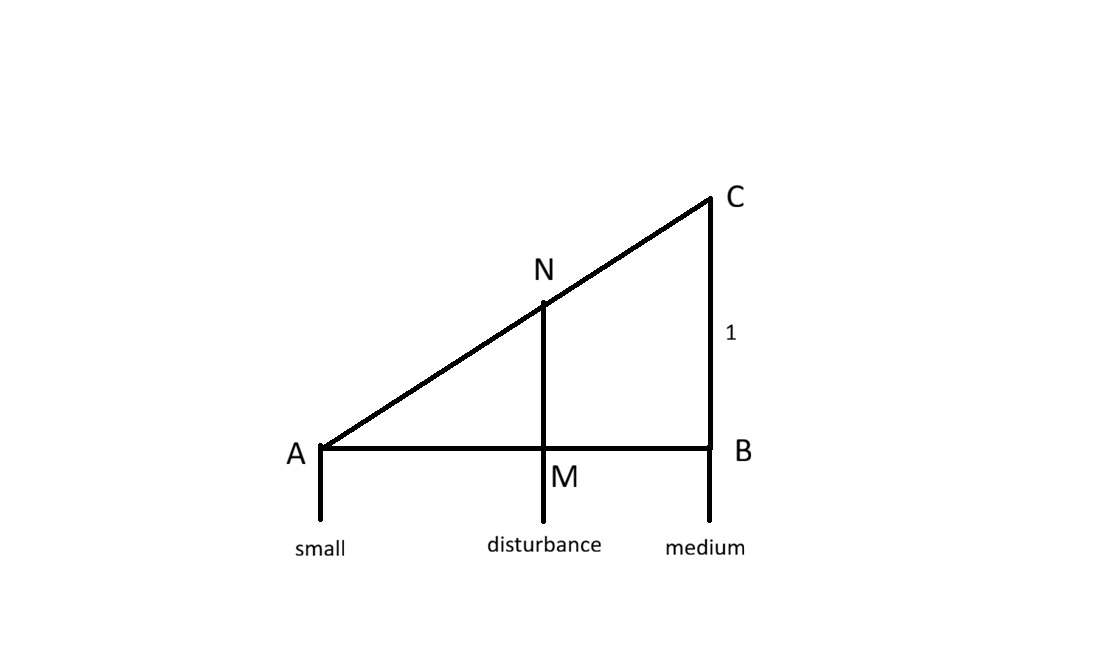
\includegraphics[width=0.7\textwidth]{images/Triangle.jpg}
    \caption{Slope of Membership Function for the Medium Fuzzy Set with a disturbance value between Small and Medium.}
    \label{fig:slope-membership-functions}
\end{figure}

This picture represents the ascending slope of the medium membership function and the disturbance having a value between small and large. It creates two similar right triangles, ABC which is formed by the full slope and AMN which is the smaller triangle formed by the membership value of the disturbance.

This means that $MN/BC$ is equal to $AM/AB$, so the side $MN = AM \times BC / AB$. Since $BC$ is equal to 1, $AM$ is disturbance $-$ small and $AB$ is medium $-$ small, the membership degree of the disturbance ($MN$) is $(\text{disturbance} - \text{small})/(\text{medium} - \text{small})$. This geometric reasoning is applied to every ascending and descending slope for each membership function in order to compute every membership value.

\subsubsection{Fuzzy Inference Rules \& Defuzzification}

\begin{lstlisting}[language=Python, caption={FuzzyPIAlgorithm inference \& defuzzification.}, label={lst:lk-init}]
def inference(self, muSmall, muMedium, muLarge):
    kpSmall = self.rules[0][0]
    kiSmall = self.rules[0][1]
    
    kpMedium = self.rules[1][0]
    kiMedium = self.rules[1][1]
    
    kpLarge = self.rules[2][0]
    kiLarge = self.rules[2][1]
    
    totalWeight = muSmall + muMedium + muLarge
    
    if totalWeight > 0:
        kpMultiplier = (muSmall * kpSmall + muMedium * kpMedium + muLarge * kpLarge) / totalWeight
        kiMultiplier = (muSmall * kiSmall + muMedium * kiMedium + muLarge * kiLarge) / totalWeight
    else:
        kpMultiplier = 1.0
        kiMultiplier = 1.0
        
    kpAdaptive = self.baseKp * kpMultiplier
    kiAdaptive = self.baseKi * kiMultiplier

    return kpAdaptive, kiAdaptive
\end{lstlisting}

The inference stage applies a set of IF-THEN rules that map each fuzzy set to specific gain multiplier values. These rules encode the control strategy: how aggressively the controller should respond to the magnitude of the disturbance. The \texttt{inference()} method handles the inference and defuzzification stages of the fuzzy control system. The Fuzzy PI algorithm uses three rules, stored in the configuration (the list Rules: $[(0.8, 0.7), (1.0, 1.0), (1.2, 1.3)]$) where each tuple represents the $K_P$ and $K_I$ multiplier for the corresponding fuzzy set.

Rule 1: IF the disturbance is small THEN $K_P \times 0.8$ and $K_I \times 0.7$. This is interpreted as: If the disturbance between the values read by the sensors is small and the robot is near the center then the gains are reduced, $K_P$ by $20\%$ and $K_I$ by $30\%$, for smooth and gentle corrections. This prevents the robot from making oscillations around the center position.

Rule 2: IF the disturbance is medium THEN $K_P \times 1.0$ and $K_I \times 1.0$. This is interpreted as: If the disturbance is medium and the robot is moderately off-center then keep the nominal gains. This is the nominal point of the controller. 

Rule 3: IF the disturbance is large THEN $K_P \times 1.2$ and $K_I \times 1.3$. This is interpreted as: If the disturbance is large and the robot is far off-center then boost the gains, $K_P$ by 20% and $K_I$ by 30% for aggressive correction. The boosted proportional gain provides immediate corrective force while the boosted integral gain helps eliminate accumulated steady-state error.

The defuzzification stage is the conversion of the fuzzy set back into a crisp value. The method mentioned previously computes a center of mass formula for defuzzification. From the inference stage, the controller combines the gain multipliers by aggregating all active rules into a pair of final adaptive gains. The denominator, being the sum of all membership values, is always equal to 1 and ensures that the result is normalized. These adaptive gains are then given to the \texttt{compute()} method to obtain the final turn rate. 

\subsubsection{Computing the Output}

\begin{lstlisting}[language=Python, caption={FuzzyPIAlgorithm output computing}, label={lst:lk-init}]
def compute(self, setPoint, measuredPoint, dt):
    disturbance=setPoint-measuredPoint
    muSmall, muMedium, muLarge=self.fuzzifyDisturbance(disturbance)
    kpAdaptive, kiAdaptive=self.inference(muSmall, muMedium, muLarge)
    
    pTerm=kpAdaptive*disturbance
    
    if dt>0:
        self.integral+=disturbance*dt
        
        if self.integral>self.fuzzyIntegralMax:
            self.integral=self.fuzzyIntegralMax
        elif self.integral<self.fuzzyIntegralMin:
            self.integral=self.fuzzyIntegralMin
            
    iTerm=kiAdaptive*self.integral
    
    output=pTerm+iTerm
    
    if output>self.fuzzyMaxOutput:
        output=self.fuzzyMaxOutput
    elif output<self.fuzzyMinOutput:
        output=self.fuzzyMinOutput
        
    return disturbance, output
\end{lstlisting}

The \texttt{compute()} method combines all stages of the fuzzy logic to obtain the final turn rate the robot must execute. It receives the \texttt{setPoint} which is usually 0, indicating perfect balance between sensors, the \texttt{measuredPoint} which is the actual difference between sensors and the change in time. The disturbance is the difference between \texttt{setPoint} and \texttt{measuredPoint}. Using the adaptive $K_P$ and $K_I$ computed from the fuzzy system, there are constructed the PI terms of the controller.

The proportional term is the product of the disturbance and the adaptive gain and acts as the correction to the current disturbance, while the integral term is the product of gain and the disturbance multiplied with the change in time, constrained by the integral interval in order to prevent the integral from growing infinitely large.

\begin{equation}
    Output=(K_P\times Imbalance)+(K_I\times\int Imbalance\ dt)
    \label{eq:kp-mult}
\end{equation}

The output final turn rate is comprised of the two PI terms and restricted to the output interval, so that the motors of the robot don’t receive impossible commands. The method returns the disturbance and the output representing the turn rate.

The \texttt{reset()} method is used to clear the integral accumulator, and it’s called whenever the controller is reinitialized. For example, after the robot handles a lane crossing event.

The advantage of this approach over a fixed-gain PID controller is that the Fuzzy PI controller automatically adjusts its output according to its position from the center. It weakens when the robot is close to the center to avoid jitters and strengthens the output when the robot is far from the center to avoid sluggish reaction to large deviations. In this behavior, the fuzzy logic provides a smooth transition between control strategies.

\subsection{Fuzzy Rule-Based Algorithm}
\label{sec:fuzzy-rb}

This algorithm relies only on fuzzy logic to control the movement of the robot based on disturbance created by the difference between values read from the sensors. Unlike the Fuzzy PI algorithm, which only tunes the gains of the PI controller, the value of disturbance and the derivative of disturbance are fuzzified and mapped through a complete Mamdani type fuzzy inference system directly to the turn rate given to the motor.

This approach has two advantages. The first one is the control strategy is expressed in natural language rules rather than mathematical gain values. This makes it easier to tune the boundaries of the fuzzy sets. The second one is by using the current disturbance and the rate of change (trend) the controller is able to anticipate future states. The correction is weakened when the robot is recovering to the center and it is strengthened when the robot begins to deviate from the center.

The algorithm is implemented in the \texttt{FuzzyRuleBased} class and comprises of the four stages of the Mamdani fuzzy controller: fuzzification of the disturbance and the trend, fuzzy inference through a set of 15 rules, aggregation of the active conclusion rules and defuzzification to obtain the crisp final turn rate.

\begin{lstlisting}[language=Python, caption={FuzzyRuleBasedAlgorithm constructor}, label={lst:lk-init}]
class FuzzyRuleBased(Algorithm):
    def __init__(self, configuration):
        self.smallDisturbance=configuration["SmallDisturbance"]
        self.mediumDisturbance=configuration["MediumDisturbance"]
        self.deltaThreshold=configuration["DeltaThreshold"]
        self.smallOutput=configuration["SmallOutput"]
        self.mediumOutput=configuration["MediumOutput"]
        self.largeOutput=configuration["LargeOutput"]
        self.rulesTable=configuration["Rules"]
        
        self.previousDisturbance=0.0
        self.firstCall = True
        self.lastActiveRules=[]
        
        self.outputSingletons=[
            -self.largeOutput,
            -self.mediumOutput,
            -self.smallOutput,
            0.0,
            self.smallOutput,
            self.mediumOutput,
            self.largeOutput,
        ]
\end{lstlisting}

The \texttt{FuzzyRuleBased} begins with the constructor, initializing from the configuration the fuzzy sets for disturbance, derivative of disturbance and the output, the interval ends restricting the output and the fuzzy rules. The interval ends are necessary to prevent the motor of the robot from executing impossible commands. The \texttt{previousDisturbance} is set to 0 to compute the derivative. The variables \texttt{firstCall}, \texttt{lastActiveRules} and \texttt{previousActiveRules} keep track of which rules are firing and by how much to debug easier. The output singletons define the magnitude of the turn rate.

\begin{lstlisting}[language=Python, caption={FuzzyRuleBasedAlgorithm clamp method}, label={lst:lk-init}]
def clamp(self, value):
        if value<0:
            return 0.0
        elif value>1:
            return 1.0
        return value
\end{lstlisting}

The \texttt{clamp()} method is a helper function which limits the range of the membership value of each fuzzy set to be between 0 and 1.

\subsubsection{Fuzzification of Disturbance}

\begin{lstlisting}[language=Python, caption={FuzzyRuleBasedAlgorithm disturbance fuzzyfication}, label={lst:lk-init}]
def fuzzifyDisturbance(self, disturbance):
    S=self.smallDisturbance
    M=self.mediumDisturbance
    
    muNL=self.clamp((-S-disturbance)/(M-S))
    
    if disturbance<=-M or disturbance>=0.0:
        muNS=0.0
    elif disturbance<=-S:
        muNS=(disturbance+M)/(M-S)
    else:
        muNS=(-disturbance)/S
        
    if disturbance<=-S or disturbance>=S:
        muZE=0.0
    elif disturbance<0.0:
        muZE=(disturbance+S)/S
    else:
        muZE=(S-disturbance)/S
        
    if disturbance<=0.0 or disturbance>=M:
        muPS=0.0
    elif disturbance<=S:
        muPS=disturbance/S
    else:
        muPS=(M-disturbance)/(M-S)
        
    muPL=self.clamp((disturbance-S)/(M-S))
    
    return (muNL, muNS, muZE, muPS, muPL)
\end{lstlisting}

The \texttt{fuzzifyDisturbance()} method takes the crisp value of the disturbance, as the first input, and computes the membership degree for each fuzzy set: negative large NL, negative small NS, zero ZE, positive small PS and positive large PL. The µNL, µNS, µZE, µPS and µPL represents the membership degrees, with values between 0 and 1 and describe how much the input resembles each set simultaneously. The reason these fuzzy sets are defined on signed disturbances, unlike the Fuzzy PI algorithm, is that this allows the controller to distinguish between left and right deviation.

These five fuzzy sets are defined by triangular and trapezoidal membership functions. They are delimited by the boundary and signed values from the configuration: -S=-3.0, -M=-6.0,  +S=3.0, +M=6.0. These boundaries determine where one fuzzy set begins and another ends, with overlapping regions where the disturbance partially belongs to two sets at the same time.  It checks for each fuzzy set because there can be more than one non-zero membership value, and that’s why the method returns all five membership values.

\begin{figure}[htbp]
    \centering
    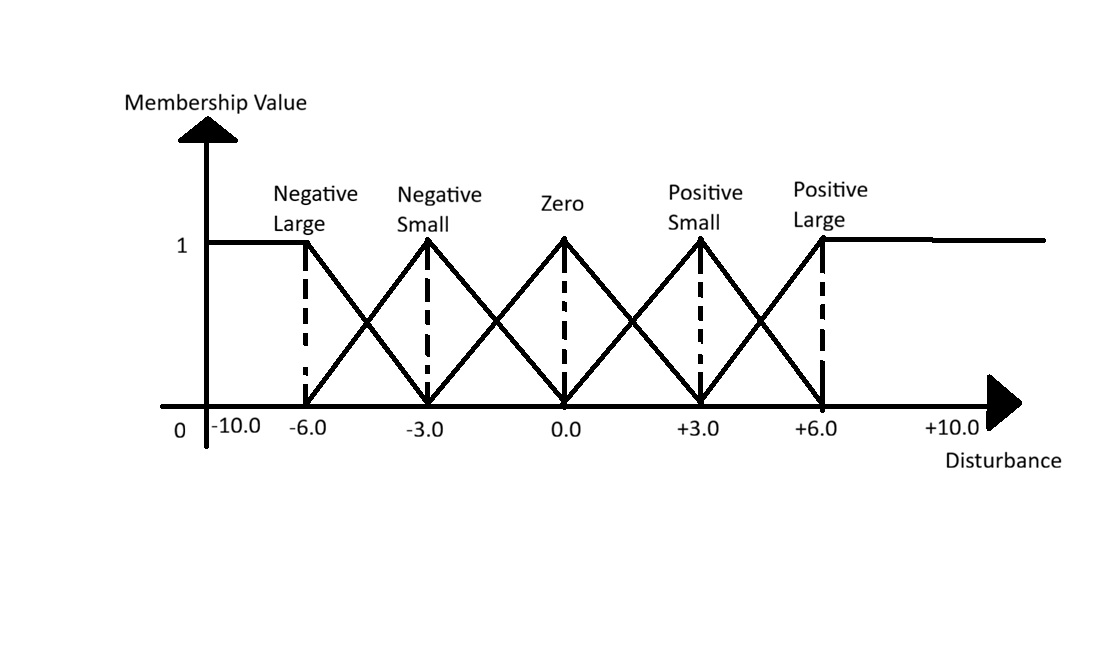
\includegraphics[width=0.7\textwidth]{images/FuzzifyDisturbance.jpg}
    \caption{Fuzzy membership functions for Small, Medium and Large disturbance sets with boundary values $S=\pm3.0$, $M=\pm6.0$ and $L=\pm10.0$.}
    \label{fig:pm-membership-functions}
\end{figure}

The picture above presents graphically the intervals where the disturbance can be situated and what membership value can have, describing a triangular/trapezoidal transition. The disturbance grows or is reduced resulting in smaller membership function for the initial set and a higher membership function for the next set.

For negative large, a trapezoidal membership function, has full membership (µNL = 1.0) when $d \le -M$. Then it decreases linearly from 1 to 0 as the disturbance increases from -M to -S. Zero membership (µNL = 0.0) when $d > -S$. This represents a strong drift to the left.

For negative small, a triangular membership function, has zero membership (µNS = 0.0) when $d < -M$ or $d > 0$. It increases linearly from 0 to 1 as the disturbance increases from -M to -S until it reaches its peak when the disturbance is exactly -S and has full membership (µNS = 1.0). Then it decreases linearly from 1 to 0 as the disturbance increases from -S to 0. This represents a slight drift to the left.

For zero, a triangular membership function, has zero membership (µZE = 0.0) when $d < -S$ or $d > +S$. It increases linearly from 0 to 1 as the disturbance increases from -S to 0 until it reaches its peak when the disturbance is exactly 0 and has full membership (µZE = 1.0). Then it decreases linearly from 1 to 0 as the disturbance increases from 0 to +S. This represents the robot being approximately centered in the lane.

For positive small, a triangular membership function, has zero membership (µPS = 0.0) when $d < 0$ or $d > +M$. It increases linearly from 0 to 1 as the disturbance increases from 0 to +S until it reaches its peak when the disturbance is exactly +S and has full membership (µPS = 1.0). Then it decreases linearly from 1 to 0 as the disturbance increases from +S to +M. This represents a slight drift to the right.

For positive large, a trapezoidal membership function, has full membership (µPL = 1.0) when $d \ge M$. It decreases linearly from 1 to 0 as the disturbance decreases from +M to +S. Zero membership (µPL = 0.0) when $d < +M$.

\begin{figure}[htbp]
    \centering
    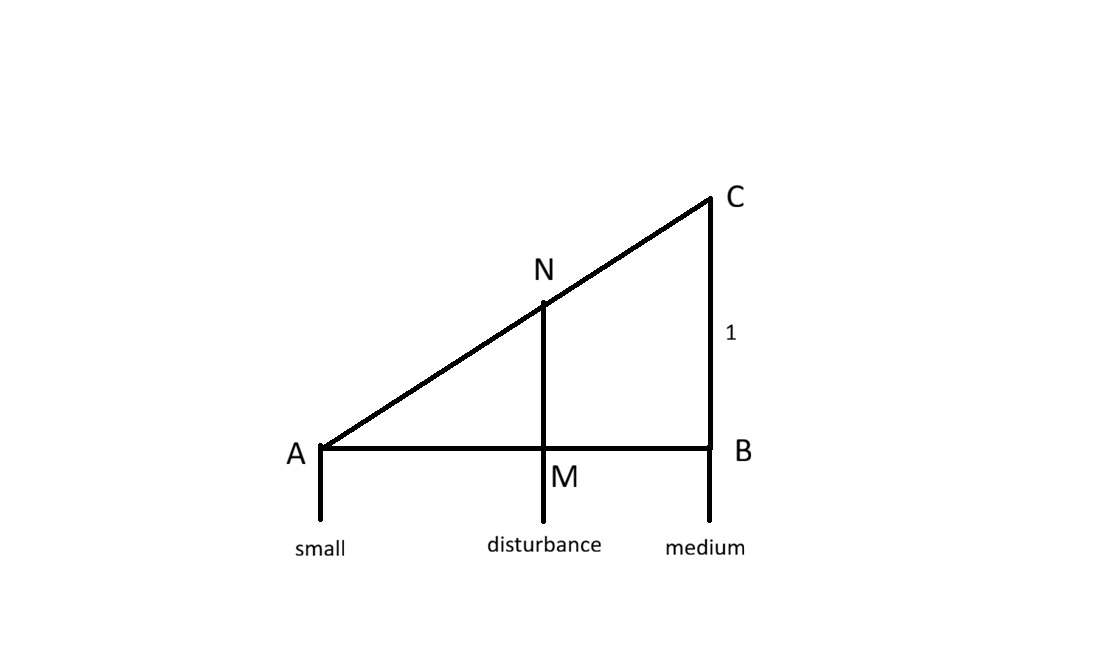
\includegraphics[width=0.7\textwidth]{images/Triangle.jpg}
    \caption{Slope of Membership Function for the Medium Fuzzy Set with a disturbance value between Small and Medium.}
    \label{fig:slope-membership-functions-frb}
\end{figure}

This picture represents the ascending slope of the medium membership function and the disturbance having a value between small and large. It creates two similar right triangles, ABC which is formed by the full slope and AMN which is the smaller triangle formed by the membership value of the disturbance. 

This means that $MN/BC$ is equal to $AM/AB$, so the side $MN = AM \times BC / AB$. Since BC is equal to 1, AM is $disturbance - small$ and AB is $medium - small$, the membership degree of the disturbance (MN) is $(disturbance\ -\ small)/(medium\ -\ small)$. This geometric reasoning is applied to every ascending and descending slope for each membership function in order to compute every membership value, as was proved for the Fuzzy PI algorithm. The trapezoidal functions have only one slope and the membership values are implemented in the code with the help from the \texttt{clamp()} method to restrict the results to the interval [0, 1], while the triangular functions have two mirrored slopes. 

\subsubsection{Fuzzification of Trend}

The second input for the fuzzy control system is how the disturbance is changing between consecutive control cycles. It is computed as $\Delta d = d_{\text{current}} - d_{\text{previous}}$. The physical interpretation of the trend depends on its sign. A positive trend means the new disturbance is higher than the previous one, so the robot is moving further from the center while a negative trend means the new disturbance is lower than the previous one, so the robot is recovering towards the center.

\begin{lstlisting}[language=Python, caption={FuzzyRuleBasedAlgorithm trend fuzzyfication}, label={lst:lk-init}]
def fuzzifyDelta(self, delta):
    D=self.deltaThreshold
    
    muN=self.clamp((-delta)/D)
    
    if delta<=-D or delta>=D:
        muZ=0.0
    elif delta<0.0:
        muZ=(delta+D)/D
    else:
        muZ=(D-delta)/D    
        
    muP=self.clamp(delta/D)
    
    return (muN, muZ, muP)
\end{lstlisting}

The \texttt{fuzzifyDelta()} method takes the crisp value of trend of disturbance. It computes the membership degree for each fuzzy set: negative N, zero Z, and positive P. The µN, µZ and µP represents the membership degrees, with values between 0 and 1 and describe how much the input resembles each set simultaneously. 

These three fuzzy sets are defined by triangular and trapezoidal membership functions. They are delimited by the threshold value from the configuration: D=3.0. 

\begin{figure}[htbp]
    \centering
    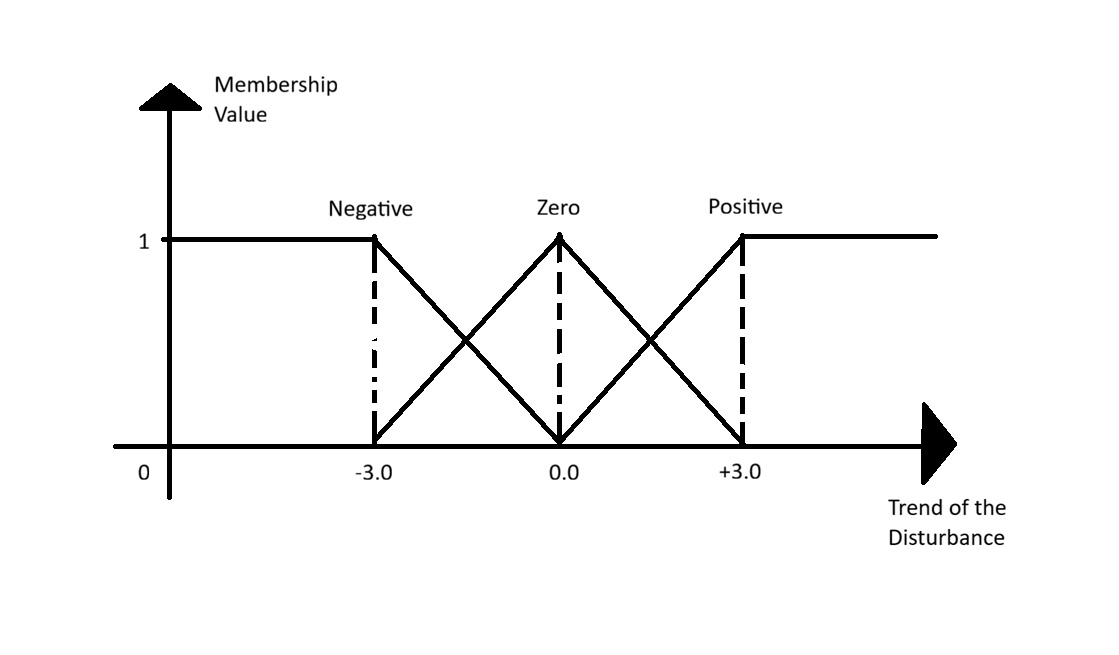
\includegraphics[width=0.7\textwidth]{images/FuzzifyTrend.jpg}
    \caption{Fuzzy membership functions for Negative, Zero and Positive trend of disturbance sets with boundary value $D=\pm3.0$.}
    \label{fig:membership-functions-trend}
\end{figure}

The picture above presents graphically the intervals where the trend of disturbance can be situated and what membership value can have, describing a triangular/trapezoidal transition.

For negative, a trapezoidal function, has full membership when $\Delta d\le -D$ and decreases linearly to 0 at $\Delta d=0$. This represents the fact that the disturbance tends to decline and the robot recovers to the center.

For zero, a triangular function, has full membership at the peak $\Delta d=0$ and decreases linearly to the base from $-D$ to $+D$. This represents a stable disturbance with little change.

For positive, a trapezoidal function, has full membership when $\Delta d\geq +D$ and decreases linearly to 0 at $\Delta d=0$. This represents the fact that the disturbance tends to grow and the robot furthers away from the center.

\subsubsection{Fuzzy Inference Rules}

The core of the Fuzzy Rule-Based controller is a set of 15 IF-THEN rules (five fuzzy sets for the disturbance and three for the trend) that map every combination of disturbance and trend to a final output turn rate. The output is expressed as seven fuzzy sets (negative large NL = -50, negative medium NM, negative NS, zero ZE, positive small PS, positive medium PM and positive large PL). Each set is associated with a singleton value that represents the magnitude of turn rate in degrees per second in the table below:

\begin{table}[htbp]
\centering
\caption{Fuzzy Rule-Based: output labels and their crisp turn rate values.}
\label{tab:rule-matrix}
\begin{tabular}{c|c|c|c|c|c|c}
\hline
\textbf{NL} & \textbf{NM} & \textbf{NS} & \textbf{ZE} & \textbf{PS} & \textbf{PM} & \textbf{PL} \\
\hline
$-50$ & $-30$ & $-10$ & $0$ & $+10$ & $+30$ & $+50$ \\
\hline
\end{tabular}
\end{table}

Negative output values command the robot to turn left, positive values command the robot to turn right and zero commands the robot to continue straight. The singleton values were chosen to express the range of the EV3 DriveBase, from gentle to aggressive corrections, while remaining below the emergency turn speed of 45 deg/s.

The 15 rules are put in a $5\times3$ matrix, whose rows correspond to the five disturbance fuzzy sets and columns to the three trend of disturbance fuzzy sets:

\begin{table}[htbp]
\centering
\caption{Fuzzy Rule-Based: rule matrix for lane keeping.}
\label{tab:rule-matrix-full}
\begin{tabular}{c|c|c|c}
\hline
\textbf{Disturbance $\backslash$ Trend} & \textbf{N} & \textbf{Z} & \textbf{P} \\
\hline
\textbf{NL} & PM & PL & PL \\
\textbf{NS} & PS & PS & PM \\
\textbf{ZE} & ZE & ZE & ZE \\
\textbf{PS} & NS & NS & NM \\
\textbf{PL} & NM & NL & NL \\
\hline
\end{tabular}
\end{table}

\begin{lstlisting}[language=Python, caption={FuzzyRuleBasedAlgorithm rules tuple}, label={lst:lk-init}]
"Rules": [
    (0, 0, 5),  # R1:  NL & N  -> PM
    (0, 1, 6),  # R2:  NL & Z  -> PL
    (0, 2, 6),  # R3:  NL & P  -> PL
    (1, 0, 4),  # R4:  NS & N  -> PS
    (1, 1, 4),  # R5:  NS & Z  -> PS
    (1, 2, 5),  # R6:  NS & P  -> PM
    (2, 0, 3),  # R7:  ZE & N  -> ZE
    (2, 1, 3),  # R8:  ZE & Z  -> ZE
    (2, 2, 3),  # R9:  ZE & P  -> ZE
    (3, 0, 2),  # R10: PS & N  -> NS
    (3, 1, 2),  # R11: PS & Z  -> NS
    (3, 2, 1),  # R12: PS & P  -> NM
    (4, 0, 1),  # R13: PL & N  -> NM
    (4, 1, 0),  # R14: PL & Z  -> NL
    (4, 2, 0),  # R15: PL & P  -> NL
],
\end{lstlisting}

The expanded rule table, encoded in the configuration as a list of tuples (disturbanceIndex, deltaIndex, outputIndex) and loaded into memory at the constructor express the IF-THEN rules and in the table below they are presented along with their physical meaning:

\begin{table}[htbp]
\centering
\caption{Fuzzy Rule-Based: full IF-THEN rule set with physical meaning.}
\label{tab:rules-full}
\begin{tabularx}{\textwidth}{c|c|c|c|X}
\hline
\textbf{Rule} & \textbf{IF disturbance is} & \textbf{AND trend is} & \textbf{THEN turn rate is} & \textbf{Meaning} \\
\hline
R1  & NL & N & PM & Far left \& recovering $\Rightarrow$ moderate right turn \\
R2  & NL & Z & PL & Far left \& stable $\Rightarrow$ strong right turn \\
R3  & NL & P & PL & Far left \& worsening $\Rightarrow$ strong right turn \\
R4  & NS & N & PS & Slightly left \& recovering $\Rightarrow$ gentle right turn \\
R5  & NS & Z & PS & Slightly left \& stable $\Rightarrow$ gentle right turn \\
R6  & NS & P & PM & Slightly left \& worsening $\Rightarrow$ moderate right turn \\
R7  & ZE & N & ZE & Centered \& recovering $\Rightarrow$ go straight \\
R8  & ZE & Z & ZE & Centered \& stable $\Rightarrow$ go straight \\
R9  & ZE & P & ZE & Centered \& worsening $\Rightarrow$ go straight \\
R10 & PS & N & NS & Slightly right \& recovering $\Rightarrow$ gentle left turn \\
R11 & PS & Z & NS & Slightly right \& stable $\Rightarrow$ gentle left turn \\
R12 & PS & P & NM & Slightly right \& worsening $\Rightarrow$ moderate left turn \\
R13 & PL & N & NM & Far right \& recovering $\Rightarrow$ moderate left turn \\
R14 & PL & Z & NL & Far right \& stable $\Rightarrow$ strong left turn \\
R15 & PL & P & NL & Far right \& worsening $\Rightarrow$ strong left turn \\
\hline
\end{tabularx}
\end{table}

The rule table has a symmetric structure with respect to 0: the output for (NL, Z) is PL (+50), while the output for (PL, Z) is NM (-50). It is equal in magnitude but opposite in sign. Similarly, (NS, Z) maps to PM (+30) and (PS, Z) maps to NM (-30). This symmetry ensures that the robot responds the same to left and right deviations.

The trend dictates the correction strength based on the situation being improved or worsened. When the trend is N (recovering) the magnitude of the correction is reduced and when the trend is P (worsening) the magnitude of the correction is increased. If the trend is Z, meaning the robot isn’t recovering yet, then the magnitude of the correction remains increased.

The centered region, when the disturbance is ZE, maps every trend to ZE keeping the robot going straight regardless of previous changes in the disturbance.

\subsubsection{Inference and Aggregation}

During each control cycle, the fuzzification stage produces up to two non-zero membership values for the disturbance from adjacent sets and up to two non-zero values for the trend. This means that at any moment, 1, 2 or 4 rules can be simultaneously active, depending on whether both inputs are exactly on a set peak (1 rule), on a transition between two sets for one input and the other is on a set peak (2 rules) or both inputs are on transitions (4 rules).

\begin{lstlisting}[language=Python, caption={FuzzyRuleBasedAlgorithm inference \& aggregation}, label={lst:lk-init}]
def inference(self, muDisturbance, muDelta):
    aggregation=[0.0]*len(self.outputSingletons)

    for disturbanceIndex, deltaIndex, outputIndex in self.rulesTable:
        ruleStrength=min(muDisturbance[disturbanceIndex], muDelta[deltaIndex])

        if ruleStrength>0.0:
            self.lastActiveRules.append((disturbanceIndex, deltaIndex, outputIndex, ruleStrength))

            if ruleStrength>aggregation[outputIndex]:
                aggregation[outputIndex]=ruleStrength

    return aggregation
\end{lstlisting}

The inference stage, implemented in the \texttt{inference()} method, firstly initializes the fuzzy output array with 0.0 activation degree for all singletons and then evaluates each of the 15 rules by computing the degree activation of the rule. The degree activation is computed by the fuzzy MIN operator, being the minimum of the two input membership values.

If one input has zero membership for a rule’s premise, the rule doesn’t activate and it’s skipped. The method keeps track of the active rules and their strength in the \texttt{lastActiveRules} list for debugging.

In the case of multiple active rules map to the same singleton output, their strength must be combined. The aggregation stage uses the fuzzy MAX operator in the way that for each output singleton, only the highest activation degree among all rules that activate it is kept. This is implemented as an array of the size corresponding to the number of singleton outputs and each entry holds the maximum degree activation for all the rules targeting that singleton.

\subsubsection{Defuzzification}

The defuzzification stage converts the aggregated fuzzy output into the crisp turn rate value. Since the output are represented as singletons, the defuzzification use center of mass formula:

\begin{equation}
    \text{turn rate} = \frac{\sum_i \text{aggregation}[i] \cdot \text{singleton}[i]}{\sum_i \text{aggregation}[i]}
    \label{eq:defuzz}
\end{equation}

\begin{lstlisting}[language=Python, caption={FuzzyRuleBasedAlgorithm defuzzification}, label={lst:lk-init}]
def defuzzify(self, aggregation):
    numerator=0.0
    denominator=0.0
    
    for i in range(len(self.outputSingletons)):
        numerator+=aggregation[i]*self.outputSingletons[i]
        denominator+=aggregation[i]
        
    if denominator>0.0:
        return numerator/denominator
    else:
        return 0.0
\end{lstlisting}

The sum collects each output singleton. Singletons with zero aggregated strengths don’t contribute to the turn rate and if no rules are active the default output is zero meaning driving straight.

\subsubsection{Computing the Output}

\begin{lstlisting}[language=Python, caption={FuzzyRuleBasedAlgorithm compute method}, label={lst:lk-init}]
def compute(self, setPoint, measuredPoint, dt):
    self.lastActiveRules=[]
    disturbance=setPoint-measuredPoint
    delta=self.updateDelta(disturbance)
    
    muDisturbance=self.fuzzifyDisturbance(disturbance)
    muDelta=self.fuzzifyDelta(delta)
    
    aggregation=self.inference(muDisturbance, muDelta)
    
    output=self.defuzzify(aggregation)
    
    return disturbance, output
\end{lstlisting}

The \texttt{compute()} method combines all stages of the fuzzy logic to obtain the final turn rate the robot must execute. It receives the \texttt{setPoint} which is usually 0, indicating perfect balance between sensors, the \texttt{measuredPoint} which is the actual difference between sensors and the change in time.

The membership values of the disturbance and delta are retrieved from the \texttt{fuzzify()} methods. Based on them, the rules are evaluated to find out which are activated in the \texttt{inference()} method. The output turn rate is defuzzified from the aggregated fuzzy sets and is clamped so that the robot doesn’t receive commands that isn’t able to execute.

% ─────────────────────────────────────────────────────────────────────────────
% 4.2  MAZE SOLVER
% ─────────────────────────────────────────────────────────────────────────────
\section{The Maze Solver Module}
\label{sec:maze-solver}

\subsection{Task Description}
\label{sec:ms-task}

This project also implements a maze-solving algorithm in which the Lego Mindstorms EV3 navigates through a maze transposed as a matrix, being discovered at runtime. The maze is composed of cells separated by walls and the robot explores every possible cell while finding a path from the starting point to the finish. The robot uses four sensors to detect its environment: an ultrasonic sensor in the front to detect the obstacles ahead, two ultrasonic sensors on the left and on the right side to balance itself in corridors and to detect open passages, and a gyroscope sensor to maintain accurate heading after turns. The forward sensor is put on a motor that rotates 90 degrees left and right to allow the robot to find the possible paths when facing a wall in the front, if there are any.

The robot drives through the maze using a Depth First Search (DFS) algorithm that maintains a map of the explored paths in memory. The robot takes each cell as a node in a graph, records visited cells and which directions are open, then explores unvisited neighbors before backtracking. This guarantees complete exploration of any connected maze. The robot stops at each junction and scans for open passages in three directions: forward, left and right. It consults the map to determine which adjacent cells are unvisited and then advances into unvisited cells or backtracks along its path to find undiscovered branches. Between junctions, the robot uses control algorithms: PID, Fuzzy PI or Fuzzy Rule-Based to regulate its forward speed based on the distance to the next wall in the front.

The architecture of this application extends the same Object-Oriented, SOLID-compliant structure from the lane keeping application. The \texttt{initializeConfiguration()} method provides all necessary variables for the maze solver task.

\begin{lstlisting}[language=Python, caption={MazeSolver task configuration}, label={lst:lk-init}]
def initializeConfiguration(task, algorithm):
    elif task == "MazeSolver":
    taskConfiguration={
        "ForwardUltrasonicSensor": Port.S4,   
        "LeftUltrasonicSensor":    Port.S1,
        "RightUltrasonicSensor":   Port.S2,   
        "GyroSensor":              Port.S3,
        "CellDistanceNS":          278,
        "CellDistanceEW":          278,
        "OpenPassageThreshold":    90,
        "ObstacleThreshold":       30,
        "TargetForwardDistance":   60,
        "BaseSpeed":               90,
        "MinSpeed":                30,
        "TurnRate":                30,
        "HeadingThreshold":        3,
        "CenteringThreshold":      20,
        "CenteringGain":           0.5,
        "CorrectionClamp":         30,
        "LogInterval":             1,
    }
\end{lstlisting}

The three ultrasonic sensors and the gyroscope sensor are assigned to their respective ports, along with the motor for the forward sensor. \texttt{CellDistanceNS} and \texttt{CellDistanceEW} represent the length and width of each cell in the maze. 
\texttt{OpenPassageThreshold} is the minimum value the sideways sensors detect in order to consider it an open path. The \texttt{ObstacleThreshold} is the distance from the wall in front so that the robot stops and checks for alternative paths. \texttt{TargetForwardDistance} is the setpoint for the control of speed algorithm. 
\texttt{BaseSpeed} is the speed of the robot while driving in a long ``corridor'' from one cell to another, while \texttt{MinSpeed} is the minimum forward velocity to prevent the robot from taking too much time to traverse a cell. The \texttt{TurnRate} is the amount of degrees to turn in one second. The \texttt{HeadingThreshold} and \texttt{CenteringThreshold} define tolerance zones for errors smaller than 3 degrees from the fixed 90 degrees turn or 20 millimeters distance from the left or right wall. The \texttt{CenteringGain} is the conversion of the lateral disturbance ($leftDistance - rightDistance$) into a corrective turn angle, capped at $\pm30$ degrees to prevent oscillation.

\subsection{The MazeMap Class}
\label{sec:mazemap}

\begin{lstlisting}[language=Python, caption={MazeMap attributes}, label={lst:lk-init}]
class MazeMap:
    NORTH = 0
    EAST  = 1
    SOUTH = 2
    WEST  = 3

    DX      = (0,  1,  0, -1)         
    DY      = (1,  0, -1,  0)          
    TURN    = (0, 90, 180, -90)        
    DFS     = (0,  3,  1,  2)          
    BACKDIR = {(0,1):0, (1,0):1, (0,-1):2, (-1,0):3}
\end{lstlisting}

The \texttt{MazeMap} class is the data structure that gives orientation and position to the robot in the maze. It keeps track of the explored cells of the maze and implements the Depth-First Search navigation logic. The class uses a coordinate system based on a compass with cardinal directions encoded as integers. The \texttt{DX} and \texttt{DY} tuples define the displacement on the x and y axis when the robot changes its position. Moving North (forward) increases y by 1, moving East (right) increases x by 1, moving South (backward) decreases y by 1 and moving West (left) decreases x by 1. The \texttt{TURN} tuple contains the rotation angles in order to face each heading direction: 0 for forward, +90 for right, 180 for backward and -90 for left. The \texttt{DFS} list contains the priority order of the directions the robot takes and the \texttt{BACKDIR} dictionary provides the reverse lookup having as key the coordinate displacement and as value the corresponding direction. 

\begin{lstlisting}[language=Python, caption={MazeMap constructor}, label={lst:lk-init}]
def __init__(self):
    self.visited           = set()
    self.path              = []      
    self.x                 = 0
    self.y                 = 0
    self.heading           = 0       
    self.expectedGyroAngle = 0
    self.cellWalls         = {}
    self.entryDirection    = None 
\end{lstlisting}

The constructor initializes the starting position of the robot with the heading towards North, an empty set of visited cells and the empty path stack, which will store the sequence of cells the robot has passed through. With this, the robot can backtrack its steps once it reaches a dead end and avoid repeating the path over and over again. 

\begin{lstlisting}[language=Python, caption={MazeMap visit method}, label={lst:lk-init}]
def markVisited(self):
    self.visited.add((self.x, self.y))
\end{lstlisting}

The \texttt{markVisited()} method adds the current cell to the visited cell. The robot will use this information to avoid going back to the same cell.

\begin{lstlisting}[language=Python, caption={MazeMap gyro target}, label={lst:lk-init}]
def gyroTarget(self):
    return self.expectedGyroAngle
\end{lstlisting}

The \texttt{gyroTarget()} method returns the expected gyroscope reading for the current heading. This is used to align the robot’s heading after turns, since the physical turn may not be perfect and the gyroscope can have some drift.

\begin{lstlisting}[language=Python, caption={MazeMap plan move method}, label={lst:lk-init}]
def planMove(self, openAbsDirs):
    for step in self.DFS:
        absDir=(self.heading + step) % 4
        
        if absDir not in openAbsDirs:
            continue
        
        nx=self.x + self.DX[absDir]
        ny=self.y + self.DY[absDir]
        
        if (nx, ny) not in self.visited:
            return absDir, self.TURN[step]
        
    return None, None
\end{lstlisting}

The \texttt{planMove()} method is the decision-making function to get the non-visited neighbouring cell. It receives as parameter the set of directions that are physically open (they are not walls) at the current junction. By iterating the DFS priority order, it checks for directions that are physically open and the cell in that direction wasn’t visited. The first direction that satisfies both conditions is returned along with the required turn angle. If there aren’t any unvisited and open directions, the method returns None and the backtracking method will be required.

The DFS priority order is defined as (0, 3, 1, 2) which translates to Forward, Left, Right and Backward. This means that the robot will continue straight until reaches a wall. It will turn left, if possible, otherwise will turn right. Finally, the robot turns around only if it’s situated at a dead end. 

\begin{lstlisting}[language=Python, caption={MazeMap plan backtrack method}, label={lst:lk-init}]
def planBacktrack(self):
    if not self.path:
        return None, None
    
    px, py=self.path[-1]
    backDir=self.BACKDIR[(px-self.x, py-self.y)]
    step=(backDir - self.heading) % 4
    
    return self.TURN[step], backDir
\end{lstlisting}

The \texttt{planBacktrack()} method handles the situation where the robot can’t navigate to other unvisited cells. It looks at the top of the path stack to retrieve the previous cell, computes the direction needed return to using the \texttt{BACKDIR} dictionary and calculates the required turn angle. If the stack is empty, the method returns None, meaning the entire maze has been explored.

\begin{lstlisting}[language=Python, caption={MazeMap apply turn method}, label={lst:lk-init}]
def applyTurn(self, absDir):
    step = (absDir - self.heading) % 4
    self.expectedGyroAngle += self.TURN[step]   
    self.heading = absDir
\end{lstlisting}

The \texttt{applyTurn()} method updates the heading before the physical turn. It calculates the turn step from the current heading to the new absolute direction and updates the expected gyroscope angle. This way the robot uses the gyroscope to align itself to the expected angle, ensuring accurate navigation through the maze.

\begin{lstlisting}[language=Python, caption={MazeMap cell information}, label={lst:lk-init}]
def storeCellInfo(self, openDirs):
        if(self.x, self.y) not in self.cellWalls:
            walls=0
            
            for direction in openDirs:
                walls |= (1 << direction)
                
            if self.entryDirection is not None:
                walls |= (1 << ((self.entryDirection + 2) % 4))
                    
            self.cellWalls[(self.x, self.y)]=walls
            
            return walls
        else:
            return None  
\end{lstlisting}    

The \texttt{storeCellInfo()} method builds and updates the map of the maze inside the robot's memory. It uses bitmasking to encode all four cardinal directions in a single integer ranging from 0 to 15. 

Firstly, the method checks its global map dictionary to see if the current cell was already stored. If it was, it returns None to avoid wasting time. Otherwise, it initializes the \texttt{walls} variable to 0. This variable serves as a 4-bit binary sequence representing the four directions: bit index 0 (value 1) = North, bit index 1 (value 2) = East, bit index 2 (value 4) = South, bit index 3 (value 8) = West.

The loop encodes the open directions by setting the corresponding bits to 1 using the left shift operator and aggregates them into the existing variable using bitwise OR. The bits of 1 represent an open path and the bits of 0 represent walls. Since the robot doesn't have a sensor in the rear, the \texttt{if} condition ensures that the robot came from an open path. \texttt{(self.entryDirection + 2)\%4} returns the opposite direction of what the robot is heading to, wrapping to values between 0 and 3. For example, if it entered heading North(0), the opposite direction is South(2). It shifts 1 to that position, forcing to register it as an open path.

Finally, it stores the resulting integer in the \texttt{cellWalls} dictionary with the current coordinates as key. This way, the robot can retrieve the information about the cell and its walls by looking up the coordinates in the dictionary.

\begin{lstlisting}[language=Python, caption={MazeMap commit move method}, label={lst:lk-init}]
def commitMove(self):
    self.entryDirection=self.heading
    self.path.append((self.x, self.y))
    self.x+=self.DX[self.heading]
    self.y+=self.DY[self.heading]
    self.markVisited()
\end{lstlisting}

The \texttt{commitMove()} method assigns the robot the current absolute direction to its entry direction in a cell, pushes the current position onto the path stack, sets the coordinates in the heading direction and marks the new cell as visited. This is called after the robot physically moves to the new cell, confirming that the move was successful and updating the state of the map.

\begin{lstlisting}[language=Python, caption={MazeMap commit backtrack method}, label={lst:lk-init}]
def commitBacktrack(self):
    self.x, self.y=self.path.pop()
\end{lstlisting}

When backtracking, the \texttt{commitBacktrack()} method pops the previous position from the path stack to restore the coordinates where the robot came from. This is called after the robot physically moves back to the previous cell, confirming that the backtrack was successful and updating the state of the map.

\subsection{The MazeSolverController}
\label{sec:ms-controller}

The \texttt{MazeSolverController} class implements the \texttt{Controller} interface and executes the DFS algorithm for the robot to traverse the maze. It handles the sensors reading, motors turning, headings aligning, centering in corridors and precise driving for distances from cell to cell.    

\begin{lstlisting}[language=Python, caption={MazeSolverController constructor}, label={lst:lk-init}]
def __init__(self, algorithm, configuration, streamer, ev3, robot, label):
    super().__init__(algorithm, configuration, streamer, ev3, robot, label)
    self.forwardSensor      = UltrasonicSensor(configuration["ForwardUltrasonicSensor"])
    self.leftSensor         = UltrasonicSensor(configuration["LeftUltrasonicSensor"])
    self.rightSensor        = UltrasonicSensor(configuration["RightUltrasonicSensor"])
    self.gyro               = GyroSensor(configuration["GyroSensor"])
    self.cellDistanceNS     = configuration["CellDistanceNS"]
    self.cellDistanceEW     = configuration["CellDistanceEW"]
    self.openPassage            = configuration["OpenPassageThreshold"]
    self.obstacleThreshold      = configuration["ObstacleThreshold"]
    self.targetForwardDistance  = configuration["TargetForwardDistance"]
    self.baseSpeed              = configuration["BaseSpeed"]
    self.minSpeed               = configuration["MinSpeed"]
    self.turnRate               = configuration["TurnRate"]
    self.headingThreshold   = configuration["HeadingThreshold"]
    self.centeringThreshold = configuration["CenteringThreshold"]
    self.centeringGain      = configuration["CenteringGain"]
    self.correctionClamp    = configuration["CorrectionClamp"]
    self.logInterval        = configuration["LogInterval"]
    self.mazeMap            = MazeMap()
\end{lstlisting}

The constructor takes the inherited attributes from the super abstract class \texttt{Controller} and adds the specific hardware for the maze: the three ultrasonic sensors, the gyroscope and the motor sensor. It instantiates the \texttt{MazeMap} object for the orientation and positioning of the robot and stores the configuration parameters for driving, turning and correction tasks. 

\begin{lstlisting}[language=Python, caption={MazeSolverController reading forward}, label={lst:lk-init}]
def scanForward(self):
    r0 = self.forwardSensor.distance()
    wait(10)
    r1 = self.forwardSensor.distance()
    wait(10)
    r2 = self.forwardSensor.distance()
    r = [r0, r1, r2]
    r.sort()
    return r[1]
\end{lstlisting}

The \texttt{scanForward()} method reads the distance from the forward ultrasonic sensor. Due to the fact that ultrasonic sensors are susceptible to spike noise caused by the echoed signals bouncing off the angled walls, the method takes three consecutive readings, sorts them and returns the median. This way, spikes are ignored. 

\begin{lstlisting}[language=Python, caption={MazeSolverController reading every direction}, label={lst:lk-init}]
def scanJunction(self):
    openDirs = set()
    h=self.mazeMap.heading
    
    if self.scanForward()>=self.openPassage:
        openDirs.add(h)
    if self.leftSensor.distance()>=self.openPassage:
        openDirs.add((h+3) % 4)
    if self.rightSensor.distance()>=self.openPassage:
        openDirs.add((h+1) % 4)
        
    return openDirs
\end{lstlisting}

The \texttt{scanJunction()} method determines which directions are open in the current cell. It receives the values read by the sensors and compares them with the \texttt{openPassage} threshold. Each value that exceeds the threshold is added to the set of open directions. The method returns this set to be passed to the \texttt{MazeMap}’s \texttt{planMove()} method for decision making.

\begin{lstlisting}[language=Python, caption={MazeSolverController gyro error computing}, label={lst:lk-init}]
def gyroError(self):
        error = self.mazeMap.gyroTarget() - self.gyro.angle()
        return (error + 180) % 360 - 180
\end{lstlisting}

The \texttt{gyroError()} method is a helper method that computes the angular error between the expected gyro target and the current gyro reading. The error is normalized to the $[{-180}^o,\ {180}^o]$ interval to ensure that the robot takes the shortest turn to align itself.

\begin{lstlisting}[language=Python, caption={MazeSolverController heading aligning}, label={lst:lk-init}]
def alignHeading(self):
    correction =self.gyroError()
    if abs(correction) > self.headingThreshold:
        self.robot.turn(correction)
        wait(20)
\end{lstlisting}

The \texttt{alignHeading()} method corrects the physical orientation of the robot to match its intended compass heading using the gyroscope. Mechanical errors such as wheel slippage can cause a deviation of the actual heading of the robot from the target, and after many turns, those accumulated errors will drive the robot into a wall. Hence, the need of this method to keep the robot from misaligning with the maze grid.

The method receives the error from the previous \texttt{gyroError()} method. If this needed correction is more than three degrees, then the robot executes a fixed turn of the computed angle and waits 20 ms for the mechanical system to settle. Otherwise, the alignment is skipped because such small corrections are within the sensor’s noise.

\begin{lstlisting}[language=Python, caption={MazeSolverController centering in corridor method}, label={lst:lk-init}]
def centerInCorridor(self):
    leftDist = self.leftSensor.distance()
    rightDist = self.rightSensor.distance()
    
    if leftDist < self.openPassage and rightDist < self.openPassage and abs(leftDist - rightDist) > self.centeringThreshold:
        correction = (rightDist - leftDist) * self.centeringGain
        
        if correction > self.correctionClamp:
            correction = self.correctionClamp
        elif correction < -self.correctionClamp:
            correction = -self.correctionClamp
        
        self.robot.turn(correction)
        wait(10)
\end{lstlisting}

The \texttt{centerInCorridor()} method adjusts the lateral position of the robot within the corridor to prevent it from driving into a side wall, using the difference between the left and right distance from the walls. If both walls are there (there is no T junction) and the difference is relevantly high, the robot executes a small corrective turn. The correction angle is computed as $difference\ \times\ centeringGain$, where this gain is 0.5 deg/mm, meaning a 100 mm offset produces a ${50}^o$ correction. The clamp acts as a protection so the robot doesn't turn to much. 

\begin{lstlisting}[language=Python, caption={MazeSolverController distance of a cell}, label={lst:lk-init}]
def cellDist(self, absDir):
    if absDir%2==0:
        return self.cellDistanceNS
    else:
        return self.cellDistanceEW
\end{lstlisting}

The \texttt{cellDist()} method returns the physical distance the robot must traverse to cross one cell in the given absolute direction. Since the maze cells are rectangular, the distance depends on whether the robot is moving along the North-South axis or the East-West axis. For the North and South directions were used even indices and odd indices were used for the East and West directions.
  
\begin{lstlisting}[language=Python, caption={MazeSolverControllerp turn executing}, label={lst:lk-init}]
def executeTurn(self, degreeTurn):
    if degreeTurn == 0:
        return
    
    if abs(degreeTurn) == 90:
        startAngle = self.gyro.angle()
        targetAngle = startAngle + degreeTurn
        deadline = self.now() + 5.0
        
        turnRate=self.turnRate if degreeTurn > 0 else -self.turnRate
        self.robot.drive(0, turnRate)
        
        if degreeTurn > 0:
            while self.gyro.angle() < targetAngle and self.now() < deadline:
                wait(10)
        else:
            while self.gyro.angle() > targetAngle and self.now() < deadline:
                wait(10)
        self.robot.stop()
    else:
        self.robot.turn(degreeTurn)
\end{lstlisting} 

The \texttt{executeTurn()} method performs the physical rotation of the robot by handling three cases:

The first case, the \texttt{degreeTurn} is  $0^o$. This means that the robot is already facing the correct direction and no action is needed.

The second case, the \texttt{degreeTurn} is ${\pm90}^o$. The method reads the starting angle from the gyro, computes the target angle and rotates with 0 linear velocity. A tight while loop continuously check the gyro sensor at a 10 ms interval until the targt heading is reached or a deadline of 5 seconds is exceeded. 

The third case treats turn-arounds where the method uses the DriveBase’s \texttt{robot.turn()} method which uses the motor encoders rather than the gyro to rotate to robot faster. 

\begin{lstlisting}[language=Python, caption={MazeSolverController cell driving}, label={lst:lk-init}]
def driveCell(self, absDir):
        cellTarget = self.cellDist(absDir)
        travelDist = 0.0
        prevSpeed  = 0.0
        lastTime   = self.now()
        self.algorithm.reset()
        wait(20)
        
        forward = self.scanForward()

        while travelDist < cellTarget and forward >= self.obstacleThreshold:
            currentTime = self.now()
            dt          = currentTime - lastTime
            lastTime    = currentTime

            forward = self.scanForward()

            if forward < self.obstacleThreshold:
                break

            disturbance, speed = self.algorithm.compute(self.targetForwardDistance, forward, dt)
            if speed < self.minSpeed:
                speed = self.minSpeed
            if speed > self.baseSpeed:
                speed = self.baseSpeed
                
            self.robot.drive(speed, 0)

            travelDist += 0.5 * (prevSpeed + speed) * dt
            prevSpeed   = speed

            self.nextStep()
            self.streamer.send(self.step, disturbance, speed)
            self.logger.log(self.step, disturbance, speed)
            
            if self.step % self.logInterval == 0:
                print("Step "+str(self.step)+" Forward: "+str(forward)+"mm Speed: "+str(speed)+" mm/s")
                if isinstance(self.algorithm, FuzzyRuleBased):
                    print(self.algorithm.logRules())
            wait(10)

        self.robot.stop()
\end{lstlisting}

The \texttt{driveCell()} method drives the robot from one cell to another using the selected control algorithm: PID, Fuzzy PI or Fuzzy Rule-Based to regulate the speed to drive forward. This is where the same algorithm classes from the lane keeping application are reused, but with the fundamental change in the algorithm’s output: for the lane keeping, the algorithm controls the turn rate to stay centered, while for the maze solver, the algorithm controls the forward speed approach the next wall safely.

At each control cycle, the forward ultrasonic sensor is read and if its value is smaller than the obstacleThreshold, the robot stops. Otherwise, the distance is passed to the algorithm’s \texttt{compute()} method. When the wall is far away, the algorithm produces a high speed, up to the base speed. As the wall gets closer to the target distance, the output speed decreases towards the minimum speed. 

The distance travelled is tracked using the velocity law: at each loop iteration, the distance increment is computed as the average between the previous and current speed multiplied with the change in time. When the integrated distance reaches the cell dimension, the robot stops and the control returns to the main DFS loop. 

The algorithm is reset at the beginning of each cell drive to clear integral accumulator and previous disturbance.

\subsection{Main Execution Loop}

\begin{lstlisting}[language=Python, caption={MazeSolverController move executing}, label={lst:lk-init}]
def executeMove(self, degreeTurn, direction, commit):
    self.executeTurn(degreeTurn)
    wait(20)
    self.mazeMap.applyTurn(direction)
    self.alignHeading()
    self.centerInCorridor()
    self.driveCell(direction)
    commit()
\end{lstlisting}

This helper method combines the low-level physical maneuvers of turning, aligning, centering and driving with structural map updates into a single high-level move execution. It receives the turn angle, the absolute direction to move and the commit function to update the map after the physical move is completed. This method is called for both forward moves and backtracking moves, since they share the same physical execution sequence.

\begin{lstlisting}[language=Python, caption={MazeSolverController run method}, label={lst:lk-init}]
def run(self):
    self.printHeader(self.algorithmLabel())
    self.gyro.reset_angle(0)
    self.mazeMap.markVisited()

    try:
        while True:
            openDirs=self.scanJunction()
            print("Cell ("+str(self.mazeMap.x)+","+str(self.mazeMap.y)+")"+" H="+str(self.mazeMap.heading)+" Open="+str(openDirs))
            
            walls=self.mazeMap.storeCellInfo(openDirs)
            if walls is None:
                walls=self.mazeMap.cellWalls.get((self.mazeMap.x, self.mazeMap.y), 0)
            self.streamer.sendCell(self.mazeMap.x, self.mazeMap.y, walls)
            
            absDir, degreeTurn=self.mazeMap.planMove(openDirs)
            
            if absDir is None:
                degreeTurn, backDir = self.mazeMap.planBacktrack()

                if degreeTurn is None:
                    print("Maze fully explored")
                    self.ev3.speaker.beep()
                    break

                print("Backtrack: turn "+str(degreeTurn)+" deg")

                self.executeMove(degreeTurn, backDir, self.mazeMap.commitBacktrack)
            else:
                print("Move: dir="+str(absDir)+" turn="+str(degreeTurn)+" deg")

                self.executeMove(degreeTurn, absDir, self.mazeMap.commitMove)
            
            self.nextStep()
            
    except KeyboardInterrupt:
        self.robot.stop()
        self.ev3.speaker.beep()
        print("\nMAZE SOLVER STOPPED at ("+str(self.mazeMap.x)+","+str(self.mazeMap.y)+")\n")
    finally:
        self.streamer.close()
        self.logger.close()
\end{lstlisting}

The \texttt{run()} method is the main execution loop that orchestrates the complete maze exploration. It combines the abstract graph traversal of the MazeMap with the physical execution of the controller. The method begins with identifying the algorithm, printing the header with the maze dimensions and threshold values, resetting the sensor motor and gyro to their zero positions and marking the the starting cell as visited. 

Then the robot scans the current junction to read forward, left and right sensors and returns the set of open directions. The open directions are passed to \texttt{storeCellInfo()} to obtain information about the current cell and pass the resulting mask to the host PC via \texttt{WifiStreamer}. 

The \texttt{planMove()} method is then called to determine the next move. If an unvisited path is found, it reurns the absolute direction and the steering rotation. The controller executes the move by calling the \texttt{executeMove()} method, passing the \texttt{self.mazeMap.commitMove} function to append the current coordinate position onto the history tracking stack.

If no unvisited direction is available, \texttt{planMove()} returns \texttt{None}. This triggers the backtrack sub-routine, invoking \texttt{planBacktrack()} to peek at the top element in the stack. It determines the rotation angle needed to step backward to its parent cell and calls \texttt{executeMove()} with the \texttt{self.mazeMap.commitBacktrack}. 

If the stack is empty, \texttt{planBacktrack()} returns \texttt{None}, which signals that the entire maze has been explored and the loop can be exited.

The loop is wrapped in a try-except block to interrupt from keyboard to stop the robot and close the WiFi stream.

\subsubsection{Fuzzy Rules for Maze Solver}
Since the \texttt{MazeSolverController} uses the same \texttt{Algorithm} interface as the \texttt{LaneKeepingController}, the same algorithms can be reused with a different interpretation of the input and output. The disturbance is still the error between the target distance and the forward sensor reading, but now the output is interpreted as a forward speed rather than a turn rate.

As such, the same PID and Fuzzy PI algorithms can be reused without modification. However, the Fuzzy Rule-Based algorithm was redesigned with a new set of rules to better suit the speed control task. The new rules are based on the distance to the wall in front and are designed to produce a smooth deceleration as the robot approaches the target distance, while maintaining a high speed when the wall is far away.

The rules are defined as follows:

\begin{table}[htbp]
\centering
\caption{Fuzzy Rule-Based: full IF-THEN rule set with physical meaning.}
\label{tab:rules-full}
\begin{tabularx}{\textwidth}{c|c|c|c|X}
\hline
\textbf{Rule} & \textbf{IF disturbance is} & \textbf{AND trend is} & \textbf{THEN speed is} & \textbf{Meaning} \\
\hline
R1  & NL & Z & PL & Far from target and far from wall\& don't care $\Rightarrow$ high speed \\
R2  & NS & Z & PL & Close to target and far from wall\& don't care $\Rightarrow$ high speed\\
R3  & ZE & Z & PM & To the target and far from wall\& don't care $\Rightarrow$ medium speed \\
R4  & PS & Z & PS & Close to target and far from wall \& don't care $\Rightarrow$ low speed \\
R5  & PL & Z & PS & Far from target and close to wall \& stable $\Rightarrow$ low speed \\
\hline
\end{tabularx}
\end{table}

These five rules are designed to take into consideration only the distance to the wall in front, since the trend of the error is not relevant for this task. The rules produce a high speed when the robot is far from the target distance. As the robot gets closer to the target, the speed decreases to medium and then low, ensuring a smooth approach to the wall without overshooting. 

The rules are implemented in the \texttt{FuzzyRuleBased} class, which uses the same fuzzification and defuzzification methods as the lane keeping version, but with the new rule set defined above. Those methods worked with two premises so these rules take the second premise the same for all to act as a neutral element. 
% ─────────────────────────────────────────────────────────────────────────────
% 4.3  THE TELEMETRY INTERFACE
% ─────────────────────────────────────────────────────────────────────────────
\section{The Telemetry Interface}
\label{sec:ui}

\subsection{WifiStreamer}
\label{sec:wifi-streamer}

\subsection{PC Receiver and Visualization}
\label{sec:pc-receiver}

% ─────────────────────────────────────────────────────────────────────────────
% 4.4  OOP ARCHITECTURE
% ─────────────────────────────────────────────────────────────────────────────
\section{Object-Oriented Architecture}
\label{sec:oop}

\subsection{Class Hierarchy}
\label{sec:class-hierarchy}

\subsection{SOLID Principles}
\label{sec:solid}

\subsection{Factory Pattern}
\label{sec:factory}

\subsection{Strategy Pattern}
\label{sec:strategy}
% ╔═══════════════════════════════════════════════════════════════════════════╗
% ║  Chapter 5 — Experimental Results                                        ║
% ╚═══════════════════════════════════════════════════════════════════════════╝
\chapter{Experimental Results}

\section{Experimental Setup}

\section{Lane Keeping Results}

\subsection{Disturbance Over Time}

\subsection{Performance Comparison}

\subsection{Turn Rate Output}

\subsection{Rule Activation Analysis}

\section{Maze Solver Results}

\subsection{Exploration Map}

\subsection{Speed Regulation}

\subsection{Maze Solver Performance}


